\bibliographystyle{babplain-fl}

\chapter{Algoritmos Aleatorizados}
\label{cha:randomized-algorithms}

  Un área activa de investigación reciente
  son los \emph{algoritmos aleatorizados}~%
    \cite{karp91:_intro_randomized_algorithms,
          motwani96:_randomized_algor}
  (fea traducción de \emph{\foreignlanguage{english}{randomized algorithms}}
   a la que nos obliga la RAE).
  En la visión tradicional de algoritmos deterministas
  nos interesan algoritmos que resuelven el problema \emph{correctamente}
  (siempre)
  y \emph{rápidamente}
  (típicamente,
   esperamos una solución en plazo polinomial en el tamaño de la entrada).
  Un algoritmo aleatorizado toma,
  además de la entrada,
  una secuencia de números aleatorios
  que usa para tomar decisiones durante la ejecución.
  Note que el comportamiento puede ser diferente
  incluso con la misma entrada.
  El interés es que en muchos casos un algoritmo aleatorizado
  es más simple
  y usa menos recursos
  (en promedio)
  que alternativas deterministas.
  Un uso importante es algoritmos aleatorizados
  para aproximar soluciones
  a problemas \NP\nobreakdash-completos.
  Véase también el capítulo~\ref{cha:algoritmos-aproximados}.
  Textos en el área son el clásico de Motwani y Raghavan~%
    \cite{motwani95:_randomized_algorithms}
  y el más accesible de Hromkovič~%
    \cite{hromkovic05:_design_anal_randomized_algor}.

\section{Clasificación de algoritmos aleatorizados}
\label{sec:clasificacion-aleatorizados}

  Los algoritmos aleatorizados se clasifican en dos grandes ramas,
  algoritmos de \emph{Monte Carlo} y \emph{Las Vegas}
  (por las famosas ciudades de juegos,
   nombres propuestos por Lázló Babai~%
     \cite{babai79:_monte_carlo_algo_graph_isomorph_test},
   en analogía a los métodos de Monte Carlo usados en análisis numérico,
   física estadística y simulación,
   aplicados ya en el proyecto Manhattan).
  Algunos hablan también de algoritmos de \emph{Atlantic City},
  otra ciudad famosa por sus casinos.

\subsection{Algoritmos de Monte Carlo}
\label{sec:algoritmos-monte-carlo}

   Un algoritmo de Monte Carlo tiene un tiempo de ejecución fijo,
   puede dar una respuesta incorrecta
   (típicamente con baja probabilidad).
   Es importante que las probabilidades y valores esperados involucrados
   son sobre las elecciones aleatorias del algoritmo,
   independientes de la entrada.
   Repitiendo el algoritmo suficientes veces
   la probabilidad de error
   disminuye exponencialmente con el número de corridas.

   Términos relevantes son \emph{errores unilaterales}
   (\emph{\foreignlanguage{english}{one-sided error}})
   y bilaterales
   (\emph{\foreignlanguage{english}{two-sided error}}).
   Un algoritmo para resolver un problema de decisión tiene error unilateral
   si siempre que se equivoca es en el mismo sentido:
   \emph{sesgo falso}
   (\emph{\foreignlanguage{english}{false biased}})
   si siempre está en lo correcto si retorna falso,
   puede equivocarse si retorna verdadero;
   \emph{sesgo verdadero}
   (\emph{\foreignlanguage{english}{true biased}})
   si siempre está en lo correcto si retorna verdadero,
   puede equivocarse si retorna falso.
   En el caso de error bilateral,
   puede equivocarse en ambas direcciones.

   Un algoritmo de Monte Carlo con sesgo falso,
   por ejemplo,
   puede usarse para determinar con alta probabilidad
   que la respuesta es \textquote{verdadero}:
   podemos correr el algoritmo suficientes veces.
   Si alguna vez responde \textquote{falso},
   sabemos que esa es la respuesta;
   si en \(n\) corridas independientes nunca responde \textquote{falso}
   sabemos con alta probabilidad que la respuesta es \textquote{verdadero}.
   En caso de un algoritmo con error bilateral,
   lo ejecutamos múltiples veces
   y quedamos con la respuesta mayoritaria.

\subsection{Algoritmos de Las Vegas}
\label{sec:algoritmos-las-vegas}

   Un algoritmo de Las Vegas
   siempre da el resultado correcto,
   pero no hay plazo definido.
   Usualmente se pide además
   que el valor esperado del tiempo de ejecución
   (dependiente de las elecciones aleatorias dentro del algoritmo)
   sea finito.

   Al analizar el tiempo de ejecución de estos algoritmos,
   este es una variable aleatoria
   (dependiente de los valores elegidos).
   Usaremos las siguientes definiciones para discutirlos.
   \begin{definition}
     \label{def:RT}
     Llamaremos \(\mathrm{RT}(u)\) al tiempo de ejecución del algoritmo
     con entrada \(u\).
   \end{definition}
   \begin{definition}
     \label{def:T-aleatorizado}
     El tiempo esperado de ejecución del algoritmo
     para entradas de tamaño \(n\) es:
     \begin{equation*}
       T(n)
         = \max_{\lvert u \rvert = n} \Exp[ \mathrm{RT}(u) ]
     \end{equation*}
   \end{definition}
   Cuidado,
   un algoritmo aleatorio puede tener tiempo máximo de ejecución
   exponencial en \(n\),
   o incluso ilimitado,
   aún si tiene buen tiempo de ejecución promedio.
   Por ejemplo,
   el tiempo de ejecución del algoritmo~\ref{alg:perder-tiempo}
   es una variable con distribución geométrica de probabilidad \(1/2\),
   con lo que,
   medido en número de invocaciones de \(\mathrm{RandBit}()\),
   es \(\Exp[\mathrm{RT}] = 2\).
   Sin embargo,
   en el peor caso nunca termina
   (si \(\mathrm{RandBit}()\) siempre retorna \num{0}).
   \begin{algorithm}[ht]
     \DontPrintSemicolon\Indp

     \While{\(\mathrm{RandBit}() = 1\)}{
       \emph{Nothing}
     }
     \caption{Perder el tiempo}
     \label{alg:perder-tiempo}
   \end{algorithm}

   Otra definición relevante es:
   \begin{definition}
     \label{def:high-probability}
     Decimos que el tiempo de ejecución del algoritmo \(A\)
     es \(O(f(n))\) \emph{con alta probabilidad}
     si hay constantes \(c > 0\) y \(d \ge 1\) tales que:
     \begin{equation*}
       \Pr[ \mathrm{RT}(A) \ge c \cdot f(n) ]
         \le \frac{1}{n^d}
     \end{equation*}
     Requeriremos también que:
     \begin{equation*}
       \Exp[ \mathrm{RT}(A) ]
         = O(f(n))
     \end{equation*}
   \end{definition}
   Note que hay varias definiciones alternativas,
   que difieren en ciertos detalles.
   Adoptaremos esta,
   mientras no haya consenso.

\subsection{Algoritmos de Atlantic City}
\label{sec:atlantic-city}

   Este término fue introducido por Finn~%
     \cite{finn82:_compar_probab_tests_primal},
   para referirse a algoritmos que dan la respuesta correcta al menos \(75\%\)
   de las veces
   (algunas otras versiones de la definición
    especifican alguna otra cota mayor a \(50\%\)).

\subsection{Primeros ejemplos}
\label{sec:randomized-examples}

  Nos interesan algoritmos más rápidos para nuestros problemas,
  posiblemente más rápidos a costa de precisión.
  Muchas veces podemos disminuir la posibilidad de error
  a tan bajo como queramos,
  aún acelerando el algoritmo.
  Los ejemplos iniciales vienen de~%
    \cite{OpenDSA16:_senior_algorithms}.

  Sabemos
  (capítulo~\ref{cha:discrete-algorithms})
  que la cota inferior para hallar el máximo
  de \(n\)~elementos no ordenados
  es \(\Omega(n)\).
  Esto es el mínimo tiempo necesario
  para asegurar que hemos identificado el máximo.
  Exploraremos cómo podemos relajar el \textquote{asegurar},
  que tiene varios aspectos.

  Hay varias garantías exigibles a un algoritmo
  que entrega \(X\) como valor máximo,
  siendo que el valor correcto es \(Y\).
  Hemos exigido \(X\) sea \(Y\).
  Esto es un algoritmo \emph{exacto} o \emph{determinista}.
  Podemos pedir solo que la posición de \(X\) en orden
  (su \emph{rango})
  es \textquote{cercano} al de \(Y\)
  (tal vez una distancia fija,
   o un porcentaje).
  Esto es un \emph{algoritmo aproximado}.
  Podemos solicitar que \(X\) \textquote{usualmente} sea \(Y\).
  Este es un \emph{algoritmo probabilístico} o \emph{aleatorizado}.
  Finalmente,
  podemos pedir
  que el rango de \(X\) \textquote{usualmente} sea \textquote{cercano}
  al rango de \(Y\).
  Esto suele llamarse \emph{algoritmo heurístico}.

  Veamos un ejemplo de algoritmo que entrega un valor grande
  dejando de lado la exigencia de obtener el mejor valor
  a cambio de mejor tiempo de ejecución.
  Es un algoritmo aleatorizado,
  en que usa el azar en su ejecución.
  Elija \(m\) elementos,
  entregue el mejor de estos como respuesta.
  Esto tiene un costo de \(m - 1\)~comparaciones
  (hay que hallar el máximo de \(m\)~elementos).
  No sabemos lo que obtendremos,
  pero podemos estimar que su rango será aproximadamente \(m n / (m + 1)\).
  Por ejemplo,
  con \(n = 1\,000\,000\) y \(m = \log n = 20\),
  esperamos que el máximo reportado pertenezca al \(5\%\)~mayor.

  Una ligera modificación es elegir un elemento en la mitad superior.
  Podemos elegir \((n + 1) / 2\) elementos y tomar el máximo de ellos,
  con un costo de \(n / 2\) comparaciones.
  Sabemos que si queremos garantía no puede hacerse mejor.
  Si estamos dispuestos a aceptar casi certeza,
  podemos hacerlo más rápido.
  Si elegimos dos elementos,
  el mayor de ellos estará en la mitad superior con probabilidad~\(3/4\)
  (no está en la mitad superior solo si ambos están en la mitad inferior).
  Si la probabilidad~\(3/4\) no es suficiente,
  ¡tome más pares!
  Para \(k\) pares,
  el máximo está en la mitad superior con probabilidad \(1 - 2^{-k}\),
  independiente del número de elementos~\(n\),
  siempre que \(n\) sea mucho mayor que~\(k\)
  (si no,
   es aún mejor).
  Con \num{10}~números,
  la probabilidad de fallar es una en~\num{1024},
  con \num{100}~números,
  la probabilidad de error es menor a la de cualquier catástrofe imaginable
  que interrumpa el proceso.

\section{Ámbitos de aplicación}
\label{sec:ambitos-aleatorizados}

% motwani96:_randomized_algor da una visión de aplicaciones más amplia

  Algoritmos aleatorizados son usados en el ámbito de teoría de números
  (el método de Miller-Rabin~%
    \cite{miller76:_Riemann_hypot_tests_primality,
          rabin80:_probab_algor_test_primality},
   un algoritmo de Monte Carlo
   para verificar primalidad,
   es el más usado actualmente).

   Una variante de Quicksort
   elige el pivote al azar,
   para hacer poco probable el peor caso
   (e incidentalmente complicarle la vida a un adversario
    que quiera forzar el peor caso).
   Estructuras de datos interesantes son
   \emph{\foreignlanguage{english}{skip lists}}~%
     \cite{pugh90:_skip_lists}
   y \emph{\foreignlanguage{english}{treaps}}~%
     \cite{aragon89:_random_search_tree,
           seidel96:_random_search_trees}
   (una mezcla de \emph{\foreignlanguage{english}{tree}}
    con \emph{\foreignlanguage{english}{heap}}),
   usan elecciones aleatorias para obtener buen rendimiento en promedio.
   Estos son todos ejemplos de algoritmos Las Vegas.

   Aplicaciones teóricas incluyen demostraciones probabilísticas de existencia:
   demostrar que un objeto con alguna característica especial
   debe aparecer con probabilidad no nula
   al elegir al azar entre una población adecuada
   demuestra que el objeto debe existir.
   Esta es la base del método probabilístico,
   que fue popularizado y aplicado ampliamente por Paul Erdős.
   Texto clásico es el de Alon y Spencer~%
     \cite{alon15:_probabilistic_method}.

   Una técnica para diseñar algoritmos deterministas
   es tomar un algoritmo aleatorizado y \textquote{desaleatorizarlo}.
   Esto es relevante en la práctica,
   pero su importancia principal
   está en desentrañar la relación
   entre las clases de complejidad correspondientes.

\section{Paradigmas de aplicación}
\label{sec:paradigmas-aleatorizado}

  Algunas de las razones que hacen útil un algoritmo aleatorizado
  son las siguientes.

\paragraph{Frustrar a un adversario}

  Si un adversario puede aprovechar el comportamiento
  de un algoritmo determinista,
  haciendo que el algoritmo tome decisiones al azar
  dificulta ataques.
  Es una posible defensa frente a \emph{ataques algorítmicos}
  (ver por ejemplo Crosby y Wallach~%
    \cite{crosby03:_DoS_algo_compl_attack}
   y McIllroy y Douglas~%
    \cite{mcillroy99:_killer_adver_quicksort}).

\paragraph{Muestreo}

  En muchos casos,
  extraemos una pequeña muestra de una gran población
  para inferir propiedades de la población.
  Computación con pequeñas muestras es barato,
  sus propiedades pueden guiar el cálculo de propiedades de la población.

\paragraph{Cualquiera sirve}

  Hay situaciones en que requerimos un objeto de características especiales,
  para los que no tenemos algoritmos eficientes que lo construyan.
  Si son comunes y simples de detectar,
  elegir al azar es una opción.

\paragraph{Abundancia de testigos}

  Muchos problemas computacionales de traducen en hallar un \emph{testigo}
  (o un certificado)
  que permita verificar una hipótesis eficientemente.
  Por ejemplo,
  para demostrar que un número es compuesto,
  basta exhibir un factor no trivial.
  Para muchos problemas,
  los testigos son parte
  de una población demasiado grande para ser revisada sistemáticamente.
  Si este espacio contiene un número relativamente grande de testigos,
  un elemento elegido al azar es probable que sea un testigo.
  Aún más,
  muestreando repetidas veces y no hallar un testigo
  disminuye exponencialmente la probabilidad de que haya un testigo,
  o sea que la hipótesis se cumple.

\paragraph{Huellas digitales}

  Una \emph{huella digital}
  (en inglés,
   \emph{\foreignlanguage{english}{fingerprint}})
  es la imagen de un elemento de un gran universo en uno mucho menor.
  Huellas digitales obtenidas mediante mapas al azar
  tienen muchas propiedades útiles.
  Veremos un par de ejemplos.

\paragraph{Reordenar al azar}

  Muchos problemas tienen la propiedad que un algoritmo bastante ingenuo
  se comporta extremadamente bien en promedio
  bajo el supuesto de datos entregados ordenados al azar.
  Aún si el algoritmo tiene mal peor caso,
  reordenar hace que el peor caso sea muy improbable.

\paragraph{Balance de carga}

  Cuando hay que elegir entre diversos recursos,
  asignar al azar
  puede usarse para \textquote{repartir} la carga en forma pareja.
  Esto resulta particularmente interesante
  cuando las decisiones deben tomarse en sistemas distribuidos,
  en forma local sin conocimiento global.

\paragraph{Aislar y quebrar simetría}

  En computación distribuida,
  es común necesitar romper un \emph{\foreignlanguage{english}{deadlock}}
  o simetría,
  o elegir un valor común
  (acordar un ordenamiento al azar de las soluciones,
   y luego buscar la primera solución por separado).

\section{Teoría de números}
\label{sec:number-theory}

  Entre las primeras aplicaciones de algoritmos probabilísticos
  se cuentan algoritmos en teoría de números.
  La teoría de números se ha hecho muy importante
  por sus aplicaciones criptográficas:
  el sistema de cifrado público RSA~%
    \cite{rivest78:_RSA}
  requiere números primos grandes,
  al igual que el intercambio de claves Diffie-Hellman~%
    \cite{diffie76:_new_directions_cryptography}.

\subsection{Preliminares teóricos}
\label{sec:nt-preliminaries}

  Si \(p\) es primo,
  el conjunto de residuos módulo \(p\) forma un campo,
  \(\mathbb{Z}_p\).
  Sabemos también que si \(x^2 = 1\) en un campo debe ser \(x = \pm 1\)
  (en nuestro caso,
   si \(p \mid x^2 - 1\) es que \(p \mid (x - 1) (x + 1)\),
   por el lema de Euclides
   \(p \mid x - 1\) o \(p \mid x + 1\)).

  El grupo de unidades \(\mathbb{Z}_p^\times\)
  (los elementos relativamente primos a \(p\),
   residuos \num{1} a \(p - 1\),
   con la multiplicación módulo \(p\))
  es cíclico,
  vale decir,
  hay un generador \(g\)
  (llamado \emph{raíz primitiva de \(p\)})
  tal que todo elemento \(a \in \mathbb{Z}_p^\times\) puede representarse como:
  \begin{equation}
    \label{eq:units-powers}
    a
      \equiv g^r
  \end{equation}
  Las raíces primitivas son relativamente frecuentes,
  es simple ver que si \(\gcd(r, p - 1) = 1\)
  entonces \(g^r\) es raíz primitiva;
  hay \(\phi(p - 1)\) raíces primitivas módulo \(p\).

  Sabemos del pequeño teorema de Fermat que para \(a \in \mathbb{Z}_p^\times\)
  es:
  \begin{equation}
    \label{eq:Fermat}
    a^{p - 1}
      \equiv 1 \pmod{p}
  \end{equation}

\subsection{Hallar números primos}
\label{sec:nt-prime-numbers}

  Si \(p\) es impar,
  \(p - 1 = q \cdot 2^s\) con \(q\) impar y \(s \ge 1\).
  Vale decir,
  \(a^{q \cdot 2^{s - 1}}\) es raíz cuadrada de \num{1},
  si es \num{1} lo es su raíz cuadrada \(a^{q \cdot 2^{s - 2}}\),
  \ldots
  Descendiendo de esta forma llegaremos a que \(a^q \equiv 1 \pmod{p}\)
  o que para algún \(0 \le k < s\) es \(a^{q \cdot 2^k} \equiv -1 \pmod{p}\).
  El contrapositivo de la observación precedente
  es que si hallamos \(a\) y \(0 \le k < s\)
  tales que \(a^{q \cdot 2^k} \equiv 1 \pmod{p}\)
  pero \(a^{q \cdot 2^{k - 1}} \not\equiv \pm 1 \pmod{p}\)
  entonces \(p\) es compuesto.
  Resulta que en tal caso a lo más una cuarta parte de los \(a\)
  mienten,
  en el sentido de dar como probable primo a un número compuesto.

  El algoritmo~\ref{alg:miller-rabin}
  es la modificación aleatorizada de Rabin~%
     \cite{rabin80:_probab_algor_test_primality}
  al algoritmo determinista de Miller~%
     \cite{miller76:_Riemann_hypot_tests_primality}.
  Supone \(p > 3\) impar.
  Generalmente se repite la prueba cierto número de veces
  para obtener mayor confianza en el resultado.
  Esta es la prueba de primalidad en más extenso uso hoy día,
  la provee por ejemplo la biblioteca LibTomMath~%
    \cite{teamtom19:_libtommath_1.2.0},
  descrita en detalle por St~Denis y Rose~%
    \cite{st_denis06:_bignum_math}.
  \begin{algorithm}
    \selectlanguage{english}
    \DontPrintSemicolon\Indp

    \Function{\(\mathrm{is\_prime}(p)\)}{
      Write \(p = q \cdot 2^s + 1\) with \(q\) odd \;
      Pick \(a\) at random from \([2, n - 2]\) \;
      \(x \gets a^q \bmod p\) \;
      \eIf{\(x = 1 \vee x = p - 1\)} {
        \Return Probably prime \;
      }{
        \For{\(k \gets 1 \KwTo s - 1\)}{
          \(x \gets x^2 \bmod p\) \;
          \If{\(x = p - 1\)}{
            \Return Probably prime \;
          }
          \Return Composite \;
        }
      }
    }
    \selectlanguage{spanish}
    \caption{Prueba de Miller-Rabin}
    \label{alg:miller-rabin}
  \end{algorithm}

\subsection{Hallar raíz primitiva módulo \(p\)}
\label{sec:nt-primitive-root}

  El intercambio de claves Diffie-Hellman~%
    \cite{diffie76:_new_directions_cryptography}
  requiere conocer una raíz primitiva \(g\) para el primo \(p\)
  para construir claves.
  No se conocen métodos eficientes para obtener una raíz primitiva
  de un primo grande,
  pero son bastante frecuentes:
  si \(g\) es raíz primitiva módulo \(p\),
  también lo es \(g^r\) siempre que \(\gcd(r, p - 1) = 1\).
  Ahora bien,
  \(g\) es raíz primitiva módulo \(p\)
  si y solo si para todos los primos \(q \mid p - 1\) es:
  \begin{equation*}
    g^{(p - 1) / q}
      \not\equiv 1 \pmod{p}
  \end{equation*}
  Un algoritmo aleatorizado para hallar un \(g\) apropiado es inmediato.

\subsection{Raíces cuadradas módulo \(p\)}
\label{sec:sqrt-mod-p}

  Es claro que si y solo si \(a \equiv g^{2 k}\)
  con \(g\) una raíz primitiva módulo \(p\)
  es un cuadrado
  (les llaman \emph{residuos cuadráticos}),
  exactamente la mitad de los elementos de \(\mathbb{Z}_p^\times\)
  es un cuadrado.
  Resulta el \emph{criterio de Euler}:
  \begin{equation}
    \label{eq:Euler-criterion}
    a^{(p - 1) / 2}
      \equiv \begin{cases}
                1 & \text{\(a\) es residuo cuadrático} \\
               -1 & \text{\(a\) es no-residuo cuadrático}
             \end{cases}
  \end{equation}
  Para referencia futura,
  al multiplicar residuos cuadráticos y no\nobreakdash-residuos cuadráticos
  da un residuo cuadrático
  si y solo si hay un número par de no\nobreakdash-residuos cuadráticos
  en el producto.

  Si \(a = 0\),
  su raíz cuadrada es \num{0}.

  En caso contrario,
  sea \(a\) un residuo cuadrático módulo \(p\),
  buscamos resolver \(x^2 \equiv a\).

  Debemos considerar varios casos.

\subsubsection{Caso \(p = 2\)}
\label{sec:p=2}

  Este caso es trivial,
  simplemente es \(\mathrm{sqrt}(a, 2) = a\).

\subsubsection{Caso \(p \equiv 3 \pmod{4}\)}
\label{sec:p-equiv-3}

  En este caso \((p - 1) / 2\) es impar,
  con lo que por el criterio de Euler:
  \begin{align*}
    a^{(p - 1) / 2}
      &\equiv 1 \\
    a \cdot a^{(p - 1) / 2}
      &\equiv a^{(p + 1) / 2} \\
      &\equiv a
  \end{align*}
  Como \(4 \mid (p + 1)\) en este caso,
  vemos que una raíz cuadrada es \(a^{(p + 1) / 4}\).

\subsubsection{Caso \(p \equiv 1 \pmod{4}\)}
\label{sec:p-equiv-1}

  Ahora \((p - 1) / 2\) es par.
  Escribamos \(p - 1 = q \cdot 2^s\) con \(q\) impar.
  Note que:
  \begin{equation*}
    \left( a^{(q + 1) / 2} \right)^2
      \equiv a^q \cdot a
  \end{equation*}
  Si \(a^q \equiv 1\),
  estamos listos.
  En caso contrario,
  tenemos \(r_0\) y \(t_0\) que satisfacen:
  \begin{equation}
    \label{eq:rt}
    r_0^2
      \equiv a t_0
  \end{equation}
  donde \(t_0 \equiv a^q\) es una raíz \(2^{s - 1}\) de \num{1},
  ya que \(t_0^{2^{s - 1}} \equiv a^{q \cdot 2^{s - 1}} \equiv a^{(p - 1) / 2}\).
  Si dados \(r_k\), \(s_k\) y \(t_k\) como en~\eqref{eq:rt}
  podemos construir un nuevo juego \(r_{k + 1}, s_{k + 1}, t_{k + 1}\)
  pero para \(s_{k + 1} = s_k - 1\),
  podemos ir reduciendo el exponente \(s\) hasta \num{0} y estamos listos.

  Si \(t_k^{2^{s_k - 2}} \equiv 1\),
  no hay nada que hacer,
  los valores anteriores sirven:
  \(r_{k + 1} = r_k\) y \(t_{k + 1} = t_k\).
  Si no,
  debe ser \(t_k^{2^{s_k - 2}} \equiv -1\),
  ya que su cuadrado es congruente con \num{1}.
  Para hallar un nuevo juego \(r_{k + 1}, t_{k + 1}\)
  multiplicamos \(r_k\) por un valor \(u\) a determinar
  tal que:
  \begin{align}
    (r_k u)^2
      &\equiv a t_k u^2 \\
      &\equiv 1 \label{eq:(ru)^2=1}
  \end{align}
  O sea:
  \begin{align*}
    r_{k + 1}
      &\equiv u r_k \\
    t_{k + 1}
      &\equiv u^2 t_k
  \end{align*}
  De~\eqref{eq:(ru)^2=1}
  vemos que \(u^2\) debe ser una raíz \(2^{s_k - 2}\) de \(-1\).
  El truco es usar un no\nobreakdash-residuo cuadrático \(b\),
  del que por el criterio de Euler sabemos:
  \begin{equation*}
    b^{q \cdot 2^{s_0 - 1}}
      \equiv -1
  \end{equation*}
  con lo que elevando \(b^q\) al cuadrado repetidas veces
  tenemos una secuencia de raíces \(2^k\) de \(-1\),
  elegimos la correcta.

  El algoritmo~\ref{alg:sqrt-mod-p} resultante es de Tonelli~%
     \cite{tonelli91:_bemerkung_aufloesung_congruenzen},
  redescubierto y mejorado casi un siglo después por Shanks~%
    \cite{shanks72:_five_number_theoretic_algorithms}.
  Es lo que provee por ejemplo la biblioteca LibTomMath~%
    \cite{teamtom19:_libtommath_1.2.0},
  descrita en detalle por St~Denis y Rose~%
    \cite{st_denis06:_bignum_math}.
  \begin{algorithm}
    \selectlanguage{english}
    \DontPrintSemicolon\Indp

    \Function{\(\mathrm{sqrt}(a, p)\)}{
      \eIf{\(p \equiv 3 \pmod{4}\)}{
        \Return \(a^{(p + 1) / 4} \bmod p\) \;
      }{
        \Repeat{\(b^{p - 1) / 2} \equiv -1 \pmod{p}\)}{
          Select \(b\) at random from \([2, (p - 1) / 2]\) \;
        }
        \tcc{\(b\) is a quadratic non-residue}
        \(q \gets (p - 1) / 4\) \;
        \(s \gets 2\) \;
        \While{\(\neg \mathrm{odd}(q)\)}{
          \(q \gets q / 2\) \;
          \(s \gets s + 1\) \;
        }
        \tcc{Now \(p - 1 = q \cdot 2^s\) with \(q\) odd}
        \(c \gets b^q \bmod p\) \;
        \(t \gets a^q \bmod p\) \;
        \(r \gets a^{(q + 1) / 2} \bmod p\) \;
        \While{\(t \not\equiv 1 \pmod{p}\)}{
          \(i \gets 1\) \;
          \(u \gets t\) \;
          \While{\(u \not\equiv 1 \pmod{p}\)}{
            \(u \gets u^2 \bmod p\) \;
            \(i \gets i + 1\) \;
          }
          \(b \gets c^{2^{s - i - 1}} \bmod p\) \;
          \(s \gets i\) \;
          \(c \gets b^2 \bmod p\) \;
          \(t \gets t b^2 \bmod p\) \;
          \(r \gets r b \bmod p\) \;
        }
        \Return \(r\) \;
      }
    }
    \selectlanguage{spanish}
    \caption{Raíz cuadrada módulo \(p\)
             (casos no triviales)}
    \label{alg:sqrt-mod-p}
  \end{algorithm}

\section{Balance de carga}
\label{sec:balance-de-carga}

  Supongamos un nuevo sitio social,
  \emph{MalaLeche}.
  Agrupa a gente dada a reclamar por todo,
  y pelearse por los temas más triviales.
  Como el tráfico es alto,
  se ha determinado que se requieren varios procesadores.
  Si alguna de las máquinas se ve sobrepasada,
  el rendimiento sufre
  (con los consiguientes reclamos de los usuarios).
  Un experimento fue asignar tareas por las primeras letras de los mensajes,
  pero peleas sobre \textquote{\textbf{pr}eferencia de editor, emacs o vi}
  y \textquote{\textbf{pr}oyecto hidroeléctrico} produjeron serios problemas.
  Si se conociera el detalle de las tareas de antemano,
  asignarlas de forma óptima entre máquinas
  es una variante del problema \textsc{Bin Packing},
  que se sabe \NP\nobreakdash-completo.
  Hay soluciones aproximadas,
  pero si no se conoce de antemano el detalle de las tareas,
  esto no tiene caso tampoco.
  Los desarrolladores abandonaron,
  y asignaron tareas al azar a las máquinas.
  Para su sorpresa,
  el sistema funciona sin problemas.

  Resulta que asignación al azar no solo balancea la carga razonablemente bien,
  también permite dar garantías de rendimiento.
  En general,
  conviene considerar un esquema aleatorizado
  si un sistema determinista es demasiado difícil
  o requiere información que simplemente no está disponible.

  Específicamente,
  MalaLeche recibe \num[group-digits = true]{24\,000} peticiones
  en cada período de \num[group-digits = true]{10} minutos.
  Se ha determinado que las peticiones
  toman a lo más \SI{1}{\second} de procesamiento;
  aunque la mayoría son triviales
  (quejarse de la ortografía del mensaje precedente
   y similares),
  siendo el tiempo promedio de ejecución \SI{0,25}{\second}.
  Midiendo el trabajo en unidades de \SI{1}{\second} de procesamiento,
  si a alguno de los servidores
  se le asignan más de \num[group-digits = true]{600} unidades de trabajo
  en \SI{10}{\minute},
  se cae y produce problemas.
  La carga total de MalaLeche
  de \(\num[group-digits = true]{24\,000}
           \cdot \num[group-digits = true]{0,25}
          = \num[group-digits = true]{6\,000}\)~unidades de trabajo
  cada \num[group-digits = true]{10} minutos
  indica que se requieren \num[group-digits = true]{10} máquinas
  trabajando al \SI{100}{\percent} con balance de carga perfecto.
  Necesitaremos más de \num[group-digits = true]{10}
  para acomodar fluctuaciones en la carga
  y balance imperfecto de carga,
  la pregunta es cuántos se requieren.

  Específicamente,
  nos interesa el número \(m\) de servidores que hace muy poco probable
  que alguno se vea sobrecargado al asignarle
  más de \num[group-digits = true]{600}~unidades de trabajo
  en un período de \num[group-digits = true]{10} minutos.

  Primero,
  acotemos la probabilidad de que el primer servidor se sobrecargue
  en un período dado.
  Sea \(T\) las unidades de trabajo asignadas a ese servidor,
  buscamos una cota superior a \(\Pr[T \ge 600]\).
  Sea \(t_i\) el tiempo que la primera máquina dedica a la tarea \(i\),
  con lo que \(t_i = 0\) si se asigna a otra máquina.
  Así,
  con \(n = \num[group-digits = true]{24\,000}\):
  \begin{equation*}
    T
      = \sum_{1 \le i \le n} t_i
  \end{equation*}
  Podemos usar las cotas de Chernoff
  (ver el apéndice~\ref{apx:pizca-probabilidades})
  si las variables son independientes
  y en el rango \([0, 1]\).
  La primera condición se cumple
  si la asignación de tareas a los servidores
  no depende de su tiempo de ejecución,
  la segunda se da porque ninguna tarea toma más de una unidad.

  Hay \num[group-digits = true]{24\,000} tareas,
  cada una de tiempo de procesamiento esperado de \(0,25\,[s]\).
  Asignado tareas al azar a los servidores,
  la carga esperada para el primer servidor es:
  \begin{align*}
    \Exp[T]
      &= \frac{\num[group-digits = true]{24\,000}
                 \cdot \num[group-digits = true]{0,25}}{m} \\
      &= \frac{\num[group-digits = true]{6\,000}}{m}
  \end{align*}
  Como vimos,
  con \(m < 10\),
  esperamos que se sobrecargue,
  con \(m = 10\) está al \SI{100}{\percent} de capacidad.

  Nos interesa el límite:
  \begin{equation*}
    600 = c \Exp[T]
  \end{equation*}
  con lo que \(c = m / 10\).
  La cota de Chernoff es:
  \begin{align*}
    \Pr[T \ge 600]
      &= \Pr\left[ T \ge \frac{m}{10} \cdot \Exp[T] \right] \\
      &\le \mathrm{e}^{-\beta(m / 10) \cdot \num[group-digits = true]{6\,000} / m}
  \end{align*}
  donde:
  \begin{equation*}
    \beta(c)
      = c \, \ln c - c + 1
  \end{equation*}
  Por la cota de la unión,
  la probabilidad de que \emph{alguna} de las máquinas
  se sobrecargue en una hora cualquiera es:
  \begin{align*}
    \Pr[\text{alguna máquina se sobrecarga}]
      &\le \sum_{1 \le i \le m} \Pr[\text{el servidor \(i\) se sobrecarga}] \\
      &=   m \Pr[\text{el servidor \num{1} se sobrecarga}] \\
      &\le m \mathrm{e}^{-\beta(m / 10) \cdot \num[group-digits = true]{6\,000} / m}
  \end{align*}
  Algunos valores se tabulan a continuación:
  \begin{center}
    \begin{tabular}[ht]{>{\(}c<{\):}>{\(}l<{\)}}
      m = 11 & 0,784\ldots \\
      m = 12 & 0,000999\ldots \\
      m = 13 & 0,0000000760\ldots
    \end{tabular}
  \end{center}
  O sea,
  con \num{11} máquinas alguna puede caerse casi inmediatamente,
  \num{12} debieran durar unos días,
  y \num{13} dan para un siglo o dos.

  Un resultado relevante es que si se revisan al azar dos de las máquinas,
  y se elige aquella con menos carga,
  la carga máxima esperada disminuye muy substancialmente
  (ver por ejemplo Mitzenmacher, Richa y Sitaraman~%
    \cite{mitzenmacher01:_power_two_random_choic}).
  Esto es importante porque no es necesario
  imponer la carga extra de revisar todas las máquinas,
  además que es fácil de hacer las consultas en paralelo.

  El resultado clásico
  (ver Gonnet~\cite{gonnet81:_expected_len_longest_probe_seq})
  es que si se distribuyen \(m\) bolas
  en \(m\) casilleros,
  con alta probabilidad el casillero más lleno contiene:
  \begin{equation*}
    (1 + o(1)) \frac{\ln m}{\ln \ln m}
  \end{equation*}
  Azar, Broder, Karlin y Upfal~%
    \cite{azar00:_balanced_alloc}
  demuestran que si hay \(m\) casilleros
  y se distribuyen \(n\)
  (\(n > m\))
  bolas entre ellos,
  si se eligen \(d\) casilleros al azar cada vez
  y se pone la bola en el más vacío
  donde \(d \ge 2\),
  el largo de la cola más larga con alta probabilidad es:
  \begin{equation*}
    (1 + o(1)) \frac{\ln \ln m}{\ln d} + \Theta(n/m)
  \end{equation*}
  La derivación es compleja,
  no la repetiremos acá.
  Vale decir,
  de \(d = 1\) a \(d = 2\) hay una mejora exponencial;
  para \(d \ge 2\) el cambio es solo en un factor constante moderado.

\section{Cotas inferiores a números de Ramsey}
\label{sec:numeros-Ramsey}

  Una aplicación del método probabilístico
  es la demostración de Erdős~%
    \cite{erdos47:_some_remarks_theo_graphs}
  de una cota inferior para el número de Ramsey \(R(r, r)\).

  El teorema de Ramsey~%
    \cite{ramsey30:_probl_formal_logic}
  en la forma que nos interesa dice que todo grafo de tamaño \(R(r, s)\)
  contiene una \emph{\foreignlanguage{english}{clique}} de tamaño \(r\)
  (un \(K_r\))
  o un conjunto independiente
  (vértices que no están unidos por arcos)
  de tamaño \(s\).
  Esto generalmente se expresa en términos de un grafo \(K_n\)
  cuyos arcos se colorean de rojo y azul,
  la pregunta es el mínimo \(n\)
  para el cual todo coloreo de arcos de \(K_n\) con rojo y azul
  tiene \(K_r\) rojo o \(K_s\) azul.
  El punto del teorema de Ramsey es que \(R(r, s)\) es finito.
  Obtener sus valores ha demostrado ser extraordinariamente difícil.

  Por ejemplo,
  tenemos el siguiente resultado:
  \begin{theorem}
    \label{theo:R(3,3)=6}
    \(R(3, 3) = 6\)
  \end{theorem}
  \begin{proof}
    Consideremos \(K_6\),
    con sus arcos coloreados de rojo o azul.
    Elija \(v\) entre sus vértices.
    Entre los \num{5} vértices restantes,
    hay al menos \num{3} unidos con arcos del mismo color a \(v\),
    digamos que es rojo.
    Si un par de estos tres vértices están conectados por un arco rojo,
    con \(v\) forman un \(K_3\) rojo.
    Si no,
    están unidos por arcos azules entre sí,
    y forman un \(K_3\) azul.
    Esto demuestra que \(R(3, 3) \le 6\).

    Por otro lado,
    la figura~\ref{fig:K5-dos-colores} muestra \(K_5\)
    con arcos coloreados de rojo y azul
    que no contiene \(K_3\) del mismo color,
    mostrando que \(R(3, 3) > 5\).
    \begin{figure}[ht]
      \centering
      % Idea for drawing filched from
      %	   http://www.texample.net/tikz/examples/combinatorial-graphs
      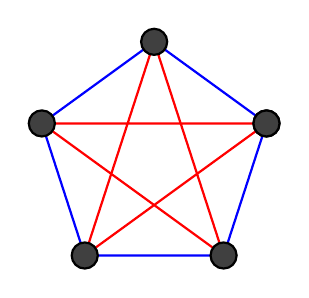
\begin{tikzpicture}[every node/.style
                            = {shape = circle, fill = black!75, draw = black}]
        \draw[thick, blue] \foreach \x in {18, 90, ..., 378}
        {
          (\x:1.5) -- (\x+72:1.5)
        };
        \draw[thick, red] \foreach \x in {18, 162, ..., 738}
        {
          (\x:1.5) node{} -- (\x+144:1.5)
        };
      \end{tikzpicture}
      \caption{\(K_5\) sin \(K_3\) monocromático}
      \label{fig:K5-dos-colores}
    \end{figure}
  \end{proof}

  Supongamos que tenemos un grafo completo \(K_n\),
  y coloreamos sus arcos de rojo y azul.
  Queremos demostrar que para valores suficientemente pequeños de \(n\)
  no hay \(r\) vértices los arcos entre los cuales son todos rojos o azules.

  Coloreemos el grafo al azar,
  asignándole el color rojo o azul a cada arco independientemente
  con la misma probabilidad.
  Calculamos el número esperado de grafos monocromáticos de \(r\) vértices
  como sigue:
  Para un conjunto \(S\) de vértices,
  sea \(X(S) = 1\)
  si todos los arcos entre vértices en \(S\) son del mismo color,
  \(X(S) = 0\) en caso contrario.
  El número de \(K_r\) monocromáticos es simplemente la suma de \(X(S)\)
  sobre todos los subconjuntos de \(r\) vértices.

  Consideremos un conjunto cualquiera \(S\) de \(r\) vértices.
  La probabilidad de que todos los arcos entre ellos
  sean del mismo color es simplemente:
  \begin{equation*}
    2 \cdot 2^{- \binom{r}{2}}
  \end{equation*}
  (el factor \num{2} es por los dos colores).
  La suma de los valores esperados de \(X(S)\) sobre todos los \(S\) es:
  \begin{equation*}
    \sum_S \Exp[X(S)]
      = \binom{n}{r} 2^{1 - \binom{r}{2}}
  \end{equation*}
  Por la linearidad del valor esperado,
  esto es:
  \begin{equation*}
    \Exp\left[ \sum_S X(S) \right]
      = \binom{n}{r} 2^{1 - \binom{r}{2}}
  \end{equation*}
  Pero esto es exactamente
  el número esperado de \(r\)\nobreakdash-subgrafos monocromáticos.

  Si este valor es menor a \num{1},
  como el número de \(K_r\) monocromáticos es un entero,
  debe haber al menos un coloreo en que es menor a \num{1}.
  Pero el único entero menor a \num{1} es \num{0}.
  O sea,
  si:
  \begin{equation*}
    \binom{n}{r}
      < 2^{\binom{r}{2} - 1}
  \end{equation*}
  hay un coloreo de los arcos de \(K_n\)
  tal que no contiene \(K_r\) rojos ni azules.

\section{Verificar producto de matrices}
\label{sec:verificar-producto-matrices}

  Supongamos que debemos verificar el producto de matrices
  \(\mathbf{A} \cdot \mathbf{B} = \mathbf{C}\).
  Usando el algoritmo tradicional con matrices de \(n \times n\)
  esto toma \(O(n^3)\) operaciones,
  el mejor algoritmo teórico da \(O(n^{2,38})\).
  El algoritmo de Freivalds~%
    \cite{freivalds77:_matrix_product_check}
  reduce esto a \(O(n^2)\).

  Elegimos \(\mathbf{a} \in \{0, 1\}^n\) uniformemente al azar,
  y calculamos \(\mathbf{A} ( \mathbf{B} \mathbf{a} )\),
  comparando con \(\mathbf{C} \mathbf{a}\).
  Esto son tres multiplicaciones de una matriz de \(n \times n\)
  por un vector de largo \(n\),
  todas demandan \(O(n^2)\) operaciones,
  y una comparación de dos vectores de largo \(n\).

  Si \(\mathbf{A} \cdot \mathbf{B} = \mathbf{C}\),
  lo anterior resulta siempre en igualdad.
  Si \(\mathbf{D} = \mathbf{A} \cdot \mathbf{B} - \mathbf{C} \ne \mathbf{0}\),
  tiene algún elemento no cero,
  digamos \(d_{i j} \ne 0\).
  Este se multiplica por \(a_i\)
  para dar
    \(\mathbf{D} \mathbf{a}
        = \mathbf{A} (\mathbf{B} \mathbf{a}) - \mathbf{C} \mathbf{a}\),
  por lo que a lo más una de las dos alternativas resultantes puede ser cero.
  O sea,
  a lo más la mitad
  de las elecciones de \(\mathbf{a}\) dice \textquote{iguales} erróneamente.
  Repitiendo \(k\) veces,
  respondiendo \textquote{distinto} si alguna vez resultan diferentes
  y \textquote{probablemente iguales} si siempre resultan iguales
  la probabilidad de error es menor a \(1 / 2^k\).
  El resultado tiene costo \(O(k n^2)\);
  y multiplicar por \(\mathbf{a}\)  no requiere multiplicaciones,
  solo sumar o no los coeficientes.

\section{Quicksort -- análisis aleatorizado}
\label{sec:quicksort-aleatorizado}

  Supongamos el siguiente modelo de Quicksort:
  estamos ordenando los valores \([1, n]\),
  antes de ordenar el arreglo los barajamos,
  y cada vez elegimos el primer elemento como pivote.
  Es un elemento al azar,
  no altera nuestro modelo.
  Definamos variables indicadoras \(X_{i j}\) para todos los pares \(i < j\)
  como \num{1} si \(i\) se compara con \(j\) durante la ejecución del algoritmo
  y \num{0} en caso contrario.
  Sorprendentemente,
  podemos calcular la probabilidad de este evento
  (y en consecuencia \(\Exp[X_{i j}]\)):
  se comparan solo si uno de los dos valores es elegido como pivote
  antes de terminar en particiones diferentes.
  Terminan en particiones diferentes si algún valor \(k\),
  con \(i < k < j\),
  se elige como pivote,
  que es exactamente si \(k\) aparece antes de \(i\) y de \(j\) en el arreglo
  al comenzar el proceso.
  Otros elementos no afectan el proceso,
  basta concentrarse en analizar permutaciones del rango \([i, j]\).
  Tenemos éxito
  (\(i\) se compara con \(j\))
  solo si la permutación de este rango comienza en \(i\) o \(j\),
  lo que ocurre con probabilidad \(2 / (j - i + 1)\),
  el valor esperado es:
  \begin{equation*}
    \Exp[X_{i j}]
       = \frac{2}{j - i + 1}
  \end{equation*}
  Sumando sobre los pares relevantes
  tenemos el número promedio de comparaciones:
  \begin{align*}
    \Exp\left[ \sum_{i < j} X_{i j} \right]
      &= \sum_{i < j} \Exp[X_{i j}] \\
      &= \sum_{1 \le i < j \le n} \frac{2}{j - i + 1} \\
      &= \sum_{1 \le i \le n - 1} \sum_{i < j \le n} \frac{2}{j - i + 1} \\
      &= 2 \sum_{1 \le i \le n - 1}
             \sum_{2 \le k \le n - i + 1} \frac{1}{k} \\
      &= 2 \sum_{1 \le i \le n - 1}
             \left( H_{n - i + 1} - 1 \right) \\
      &= 2 \sum_{1 \le i \le n - 1} H_{n - i + 1} - 2 (n - 1) \\
      &= 2 \sum_{2 \le k \le n} H_k - 2 (n - 1) \\
      &= 2 \sum_{1 \le k \le n} H_k - 2 n \\
      &= 2 \left( (n + 1) H_n - n \right) - 2 n \\
      &= 2 (n + 1) H_n - 4 n
  \end{align*}
  Igual que lo que obtuvimos antes~\eqref{eq:quicksort-comparisons}.

  Pero podemos ir más allá.
  Supongamos que corremos Quicksort aleatorizado
  sobre un arreglo de \(n\) elementos
  y paramos la recursión a profundidad \(c \ln n\) para una constante \(c\).
  La pregunta es cuál es la probabilidad
  que haya una hoja del árbol de llamadas
  al que no le corresponde ordenar un rango de un único elemento.
  Llame una división
  (inducida por un pivote)
  \emph{buena} si divide el conjunto \(S\) en pedazos \(S_1\) y \(S_2\)
  tales que:
  \begin{equation*}
    \min\{ \lvert S_1 \rvert, \lvert S_2 \rvert \}
      \ge \frac{1}{3} \lvert S \rvert
  \end{equation*}
  Si no es así,
  la llamamos \emph{mala}.
  Con nuestra suposición que todos los elementos son diferentes,
  vemos que la probabilidad de una buena división es \(1/3\).

  Cada buena división reduce el tamaño de la partición
  por un factor de al menos \(2/3\).
  Para llegar a un rango de un único elemento requerimos:
  \begin{align*}
    k
      &= \frac{\ln n}{\ln (3/2)} \\
      &= a \ln n
  \end{align*}
  buenas divisiones.
  Interesa ahora qué tan grande debe ser \(c\)
  para que la probabilidad de menos de \(a \ln n\) buenas divisiones
  sea pequeña.

  Consideremos el camino de la raíz a una hoja del árbol de recursión.
  Divisiones sucesivas son buenas o malas independientemente,
  podemos usar la cota de Chernoff:
  \begin{align*}
    \Pr\left[
         \text{número de buenas divisiones}
            < \frac{1}{3} a \ln n
        \right]
      &\le \mathrm{e}^{- \beta(1 / c) \cdot \frac{1}{3} c a \ln n} \\
      &= n^{- \beta(1 / c) c a / 3}
  \end{align*}
  Podemos elegir \(c\) de manera que \(\beta(1 / c) c a / 3 \ge 2\)
  (con \(c = 6\) tenemos de sobra).

  Por lo anterior,
  la probabilidad que en \emph{una} rama
  hayan muy pocas divisiones buenas es a lo más \(n^{-2}\);
  como hay a lo más \(n\) ramas,
  por la cota de la unión
  esto significa que la probabilidad
  que en \emph{alguna} rama hayan pocas divisiones buenas
  es a lo más \(n^{-1}\).
  Pero esto es la probabilidad que tome más de \(O(n \log n)\) comparaciones,
  y Quicksort aleatorizado ejecuta \(O(n \log n)\) comparaciones
  con alta probabilidad.

\section{Comparar por igualdad}
\label{sec:comparar}

  Supongamos que tenemos un gran archivo,
  por ejemplo medios de instalación de su distribución favorita,
  y quiere verificar que no contiene errores,
  vale decir,
  coincide con la versión original.
  Obviamente,
  queremos hacer esto sin demasiado cómputo adicional
  (somos impacientes)
  ni usando demasiado tráfico de red
  (somos amarretes).
  Omitiendo consideraciones criptográficas,
  el problema es calcular alguna forma
  de \emph{\foreignlanguage{english}{checksum}},
  tarea para la cual hay soluciones estándar,
  como CRC
  (\emph{\foreignlanguage{english}{Cyclic Redundancy Check}},
   inventado por Peterson~%
     \cite{peterson61:_CRC};
   un rápido resumen da por ejemplo Williams~%
     \cite{williams96:_painless_guide_crc}).

  Concretamente,
  supongamos que el archivo de marras es de \(n\)~bits,
  el original es \(\langle a_1, a_2, \dotsc, a_n \rangle\),
  la copia local es \(\langle b_1, b_2, \dotsc, b_n \rangle\).
  Algoritmos de \emph{\foreignlanguage{english}{checksum}} estándar
  garantizan
  que para la \textquote{mayoría} de los vectores \(\mathbf{a}\) y \(\mathbf{b}\)
  van a detectar si no son iguales.
  Acá la garantía
  es sobre una distribución de \(\mathbf{a}\) y \(\mathbf{b}\).
  Para los algoritmos comunes hay técnicas para \textquote{falsificar} CRC
  (ver por ejemplo Stigge y otros~%
     \cite{stigge06:_reversing_crc}),
  con lo que esto no es suficiente.
  Nos interesa únicamente acotar el tráfico de datos
  entre el origen y nosotros,
  el costo de cómputo es secundario.

  Nos interesa analizar el peor caso,
  interesa una garantía de la forma:
  para \emph{todo} par de vectores \(\mathbf{a}\) y \(\mathbf{b}\),
  elegiremos algunos valores al azar,
  y para la mayoría de los valores elegidos el algoritmo
  detectará si hay diferencias.
  Esta garantía no depende de \textquote{buenos} o \textquote{malos} vectores
  \(\mathbf{a}\) y \(\mathbf{b}\),
  solo de posiblemente \textquote{malos} valores elegidos.

  Nuestro algoritmo se basa en considerar los vectores
  como coeficientes de polinomios sobre un campo finito \(\mathbb{F}_p\).
  Recordemos el siguiente teorema
  (ver el apunte de Fundamentos de Informática~%
    \cite[sección~9.3]{brand17:_fundamentos_informatica}):
  \begin{theorem}
    Sea \(f(x)\) un polinomio no-cero de grado a lo más \(d\)
    sobre un campo.
    Entonces \(f\) tiene a lo más \(d\) ceros
    (hay a lo más \(d\) valores de \(x\) en el campo tales que \(f(x) = 0\)).
  \end{theorem}
  El primer paso es elegir un primo \(p \in [2 n, 4 n]\)
  (el postulado de Bertrand~%
     \cite{erdos30:_beweis_satz_tschebyschef}
   asegura que entre \(m\) y \(2 m\) siempre hay un primo,
   podemos buscar en el rango hasta hallar uno;
   los primos son relativamente numerosos,
   esto no es demasiado costoso).
  Enseguida,
  construya los polinomios sobre \(\mathbb{F}_p\):
  \begin{align*}
    a(x)
      &= \sum_{1 \le k \le n} a_k x^k \\
    b(x)
      &= \sum_{1 \le k \le n} b_k x^k
  \end{align*}
  Sea \(g(x) = a(x) - b(x)\).
  Note que \(g(x)\) es el polinomio cero
  si y solo si \(\mathbf{a} = \mathbf{b}\);
  si \(\mathbf{a} \ne \mathbf{b}\),
  \(g(x)\) es un polinomio de grado a lo más \(n\),
  que tiene a lo más \(n\) ceros.
  Si seleccionamos \(x \in \mathbb{F}_p\) uniformemente al azar,
  la probabilidad que \(g(x) = 0\) es a lo más:
  \begin{equation*}
    \frac{n}{\lvert \mathbb{F}_p \rvert}
      = \frac{n}{p}
      \le \frac{1}{2}
  \end{equation*}

  Esto sugiere el algoritmo~\ref{alg:comparar-archivos}.
  \begin{algorithm}[ht]
    \DontPrintSemicolon\Indp

    Agree on prime \(p\) with the origin \;
    \(k \gets 0\) \;
    \For{\(k \gets 1\) \KwTo \(m\)}{
      Origin selects \(x \in \mathbb{F}_p\) uniformly at random
        and computes \(a(x)\) \;
      Origin sends \(x\) and \(a(x)\) \;
      Destination computes \(b(x)\) \;
      \If{\(a(x) \ne b(x)\)}{
        \Return Different \;
      }
    }
    \Return Probably equal \;
    \caption{Comparar archivos remotos}
    \label{alg:comparar-archivos}
  \end{algorithm}

  Vemos que este algoritmo nunca dice \textquote{diferentes} por equivocación,
  se equivoca cada vez a lo más \(1/2\) de las veces,
  en \(m\) iteraciones la probabilidad de error es a lo más \(2^{-m}\).
  Intercambiamos \(m\) números en \([2 n, 4 n]\),
  el tráfico total es \(O(m \log n)\).

  Otra opción es elegir \(p \in [ r n, 2 r n]\),
  lo que con una iteración da probabilidad de falla a lo más \(1/r\),
  si esto es \(2^{-m}\) es \(r = 2^m\)
  y los bits intercambiados
  son \(O(\log p) = O(\log n + \log r) = O(\log n + m)\),
  mejor que lo anterior.

  Lo que discutimos acá es un ejemplo de lo que Karp~%
    \cite{karp91:_intro_randomized_algorithms}
  llama \emph{\foreignlanguage{english}{fingerprinting}},
  representar una estructura grande y compleja
  por una huella digital pequeña.
  Si dos estructuras tienen la misma huella digital,
  es fuerte evidencia de que en realidad son iguales.
  Una huella elegida al azar dificulta ataques o coincidencias,
  y puede repetirse para aumentar la confianza.

\section{Patrón en una palabra}
\label{sec:patron}

  Una tarea común es determinar si un patrón \(\sigma\)
  aparece en una palabra \(\omega\).
  El algoritmo obvio compara el patrón en cada posición de \(\omega\),
  dando un algoritmo determinista cuadrático
  (\(O(\lvert \sigma \rvert \cdot \lvert \omega \rvert)\)).
  Hay algoritmos deterministas lineales
  (\(O(\lvert \sigma \rvert + \lvert \omega \rvert)\)),
  como el de Knuth-Morris-Pratt~%
    \cite{knuth77:_fast_pattern_match_strings}
  y el de Boyer-Moore~%
    \cite{boyer77:_fast_string_search_algor}
  con la modificación de Galil~%
    \cite{galil79:_improving_worst_case_running_time},
  pero son muy complicados.

  Discutiremos el algoritmo de Karp y Rabin~%
    \cite{karp87:_efficient_random_pattern_match_algor}.
  Sigue la idea de fuerza bruta de ubicar el patrón en cada posición,
  pero en vez de comparar el patrón con la palabra compara una huella digital,
  fácil de calcular y de actualizar.
  Para simplificar lo que viene,
  sean \(n = \lvert \sigma \rvert\)
  y \(m = \lvert \omega \rvert\).
  Sea también \(b \ge \lvert \Sigma \rvert\) una base conveniente.
  Usaremos por ejemplo \(\omega_i\)
  para representar el \(i\)\nobreakdash-ésimo símbolo de \(\omega\).
  Para abreviar,
  anotaremos además \(\omega_{[i, j]}\)
  para referirnos al rango \(\omega_i \omega_{i + 1} \dots \omega_j\).
  Sea \(p\) un primo,
  elegido al azar en el rango \([1, n m^2]\).
  Usamos la huella digital
  (nuestras operaciones son en \(\mathbb{Z}_p\)):
  \begin{equation*}
    h(\sigma)
      = \sigma_1 \cdot b^{n - 1}
          + \sigma_2 \cdot b^{n - 2}
          + \dotsb
          + \sigma_n
  \end{equation*}
  Lo crítico
  es que es fácil actualizar \(h\) al eliminar el primer símbolo
  y agregar uno nuevo:
  \begin{equation*}
    h(\omega_{[i + 1, i + n]})
      = (h(\omega_{[i , i + n - 1]}) - \omega_i b^{n - 1})
           \cdot b + \omega_{i + n}
  \end{equation*}
  Esto da lugar al algoritmo~\ref{alg:Karp-Rabin}.
  \begin{algorithm}[ht]
    \DontPrintSemicolon\Indp

    Select \(p\) at random as indicated \;
    \BlankLine
    \(h \gets 0\) \;
    \For{\(k \gets 1\) \KwTo \(n\)}{
      \(h \gets h \cdot b + \sigma_k\) \;
    }
    \BlankLine
    \(s \gets 0\) \;
    \For{\(k \gets 1\) \KwTo \(n\)}{
      \(s \gets s \cdot b + \omega_k\) \;
    }
    \BlankLine
    \(k \gets n\) \;
    \While{\((s \ne h) \wedge (k < m)\)}{
      \(k \gets k + 1\) \;
      \(s \gets (s - \omega_{k - n} \cdot b^{n - 1}) \cdot b
                       + \omega_k\) \;
    }
    \eIf{\(s = h\)}{
      \Return Probable match at \(k - n\) \;
    }{
      \Return No match \;
    }
    \caption{El algoritmo de Karp-Rabin para calces de patrones}
    \label{alg:Karp-Rabin}
  \end{algorithm}
  Podemos verificar probables calces comparando símbolo a símbolo.

  Si \(h(\alpha) \ne h(\beta)\),
  es claro que \(\alpha \ne \beta\).
  Nos interesa el caso en que \(\alpha \ne \beta\),
  pero \(h(\alpha) = h(\beta)\).
  Un adversario que conoce el funcionamiento de nuestro algoritmo y \(p\)
  podría elegir \(\beta\) para forzar esto en muchas posiciones,
  haciendo que debamos recurrir a comparaciones inútiles
  (llegando a tiempo \(O(n m)\)).
  % Completar el análisis... ver el paper de Karp-Rabin
  %   karp87:_efficient_random_pattern_match_algor

% To do:
% Binary Planar Partition, autopartition ~~-> presentación de Raghavan
%  raghavan:_randomized_algorithms
% More algorithms (Karger, skip lists, max cut)
% Exercises!

\bibliography{../referencias}

%%% Local Variables:
%%% mode: latex
%%% TeX-master: "../INF-221_notas"
%%% ispell-local-dictionary: "spanish"
%%% End:

% LocalWords:  Aleatorizados aleatorizados english randomized Carlo
% LocalWords:  algorithms polinomial aleatorizado Lázló Babai City em
% LocalWords:  Manhattan Atlantic one sided two biased ht heurístico
% LocalWords:  probabilístico primalidad Quicksort skip lists treaps
% LocalWords:  tree heap probabilísticas Paul Alon Spencer Crosby RSA
% LocalWords:  desaleatorizarlo muestreando fingerprint Reordenar St
% LocalWords:  reordenar deadlock probabilísticos contrapositivo with
% LocalWords:  LibTomMath Write odd Pick at random from Probably Now
% LocalWords:  Composite redescubierto Select quadratic residue pr RT
% LocalWords:  MalaLeche eferencia emacs oyecto Bin Packing clique eq
% LocalWords:  linearidad subgrafos permutaciones permutación CRC rt
% LocalWords:  recursión amarretes checksum Cyclic Redundancy Check
% LocalWords:  fingerprinting ésimo false true Nothing aleatorizada
% LocalWords:  ru is quicksort comparisons Agree on the origin and
% LocalWords:  selects uniformly sends Destination Different equal
% LocalWords:  indicated match
